% ==============================================================
% --- Git
% ==============================================================
\section{Collaborative Software Development}\hypertarget{sec3}{}

\begin{frame}[fragile]
\emptyframetitle
  In this section
  \begin{itemize}
    \item \hyperlink{sec3.1}{Creating Remote Repositories on GitHub}
    \item \hyperlink{sec3.2}{Collaborating On GitHub}
    \item \hyperlink{sec3.3}{Conflicts}
  \end{itemize}
\end{frame}

\subsection{Creating Remote Repositories on GitHub}\hypertarget{sec3.1}{}

\begin{frame}[fragile]
\emptyframetitle
  One of the main reasons for using repositories is also to \textbf{collaborate with other people} and \textbf{work on the same code}. This is done through a \textbf{remote repository}. \\[0.25cm]

  \textbf{\textit{Pulling} retrieves from} the remote repo.\\
  \textbf{\textit{Pushing} deposits into} the remote repo.\\
  \textbf{\textit{Cloning} checks out a private copy} of the remote repo.
  \begin{figure}[h]
    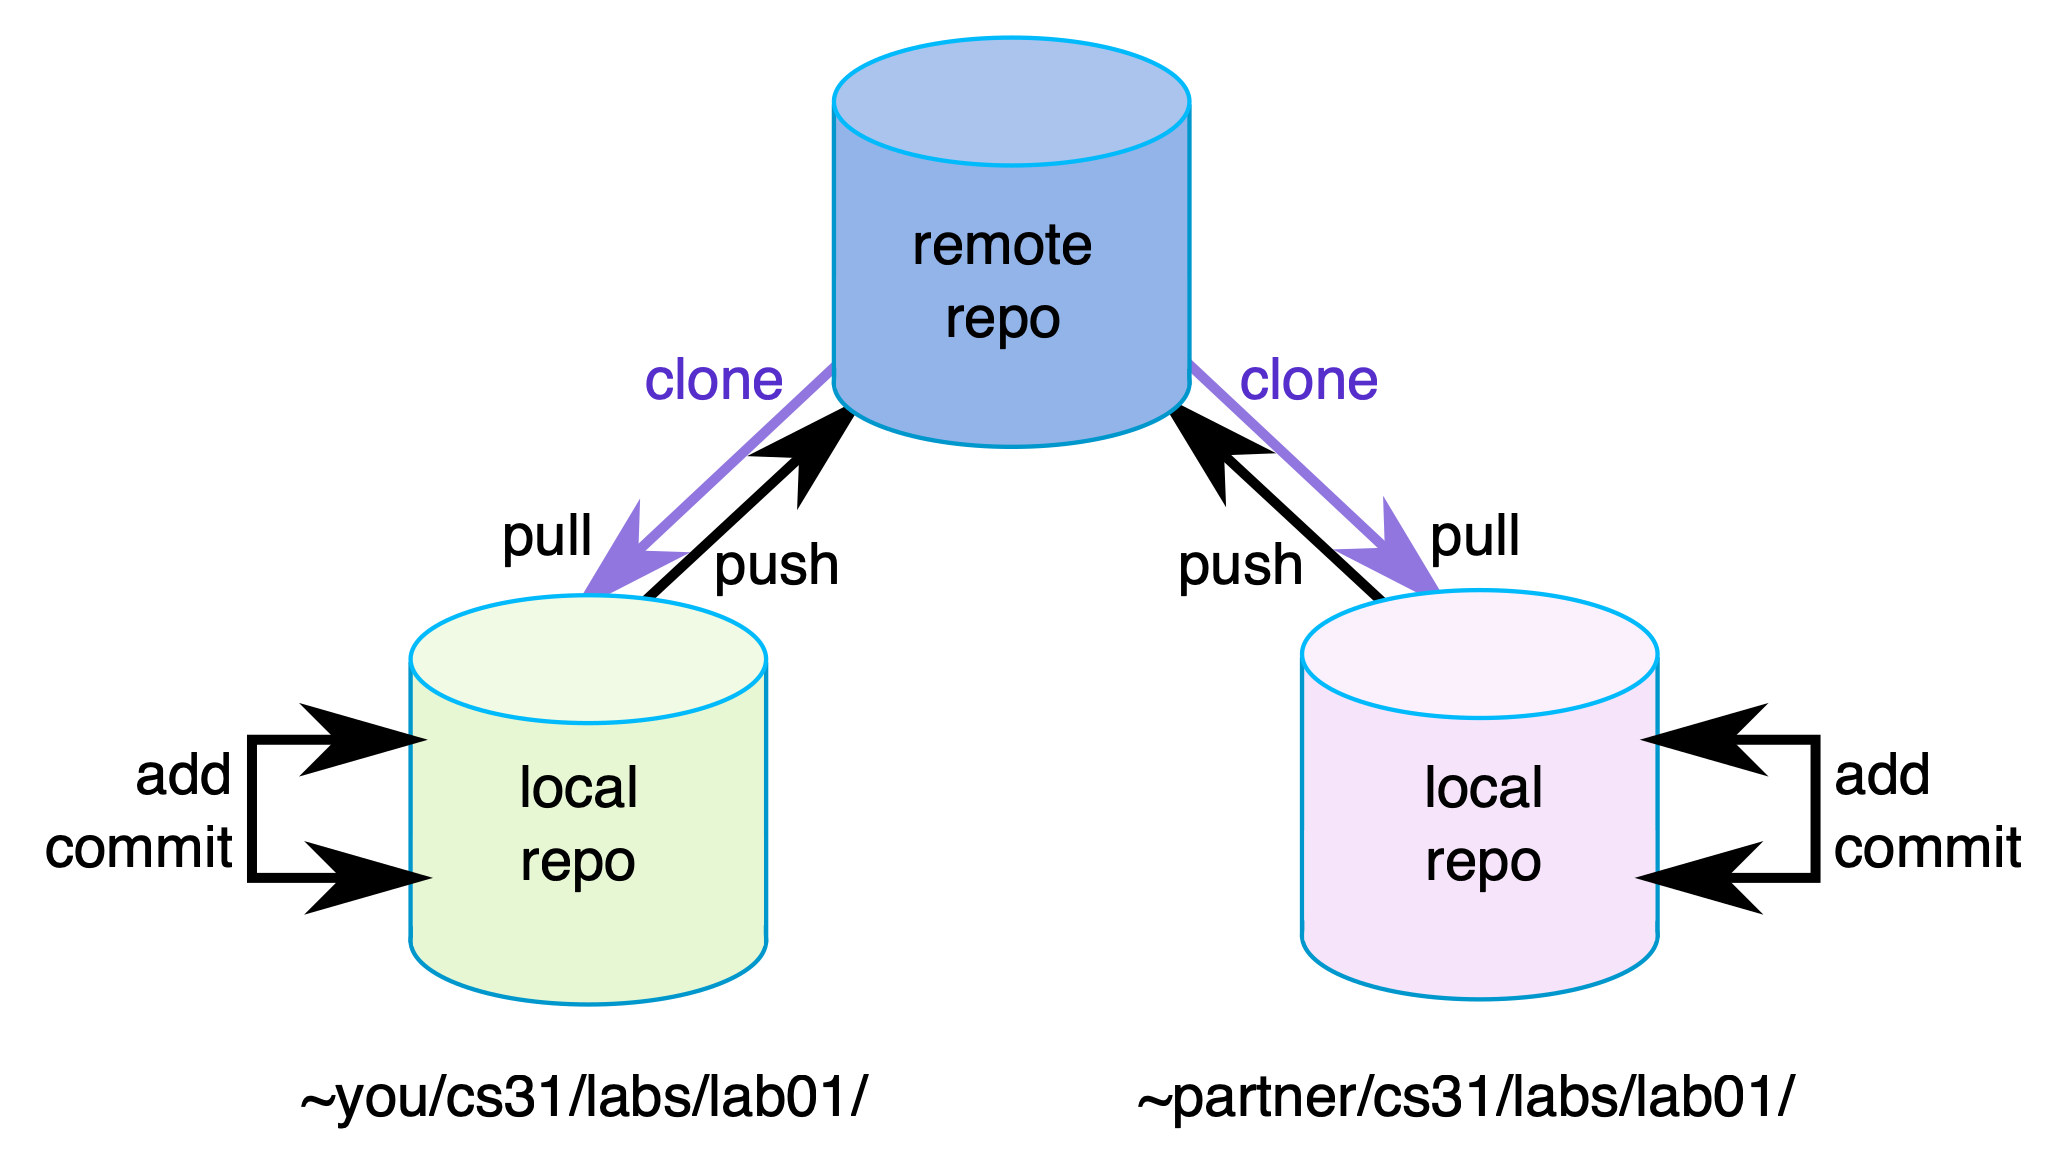
\includegraphics[width=0.7\textwidth]{sec3/git-repo_overview.png}
  \end{figure}

\end{frame}

\begin{frame}[fragile]
\emptyframetitle
  We will use \textbf{GitHub} available at \textbf{\url{https://github.com}}

  \begin{figure}[h]
    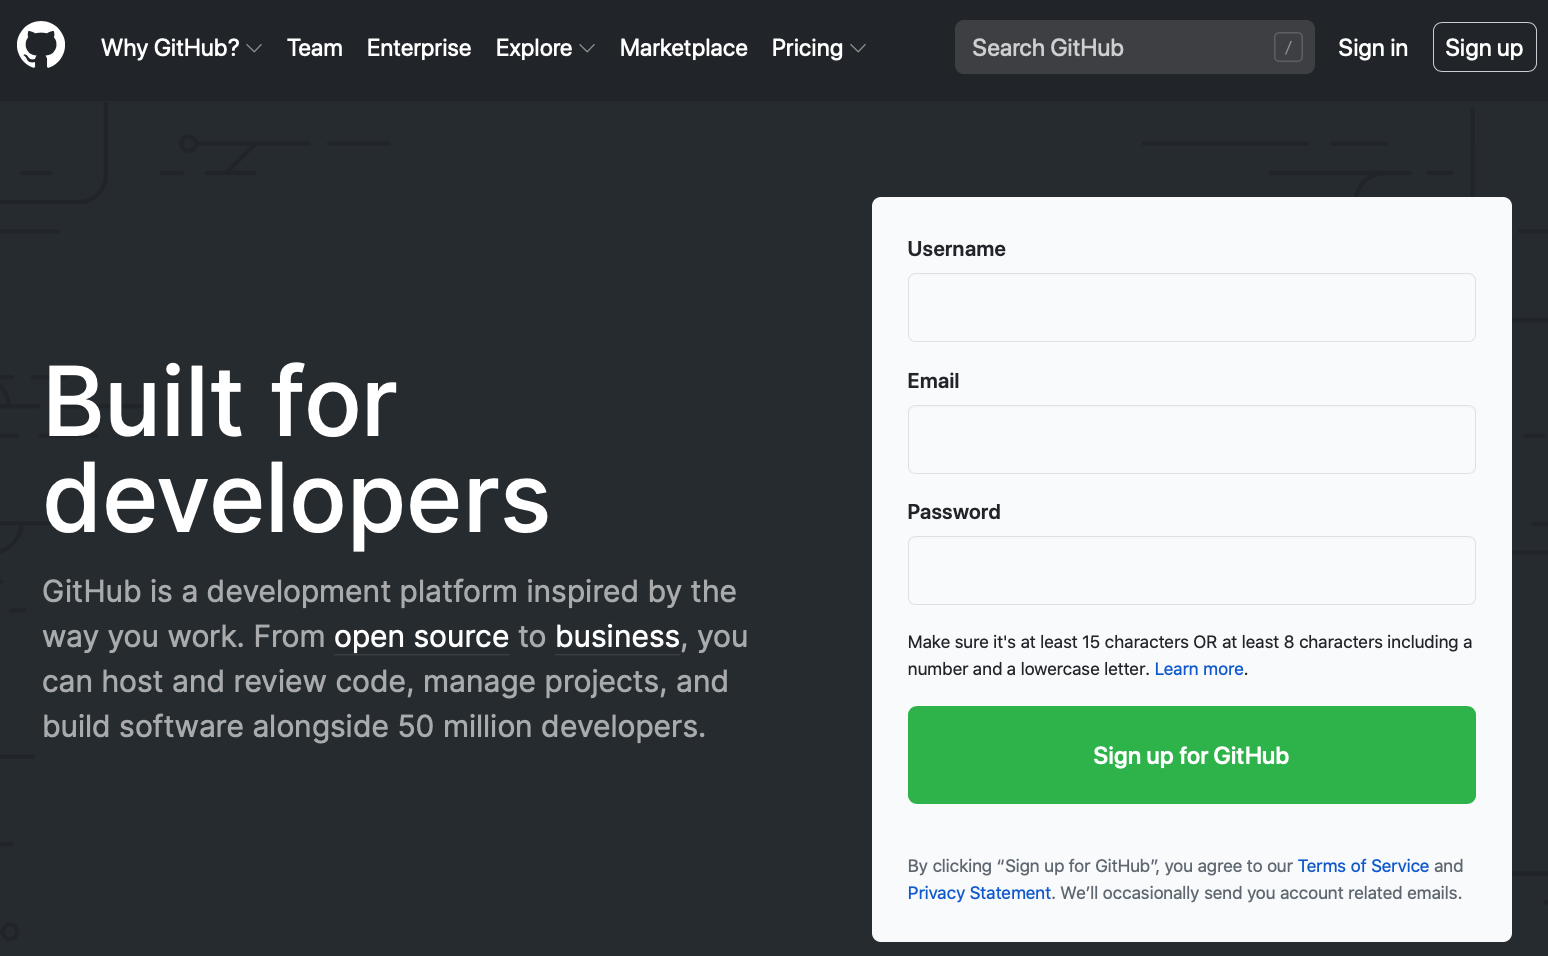
\includegraphics[width=0.75\textwidth]{sec3/github-signup.png}
  \end{figure}

  Pick a username and sign up now with one of your email addresses.

\end{frame}

\begin{frame}[fragile]
\emptyframetitle

  Once you have an account, go to your profile page. This is in the drop-down menu under the avatar in the top right-hand corner.
  \begin{figure}[h]
    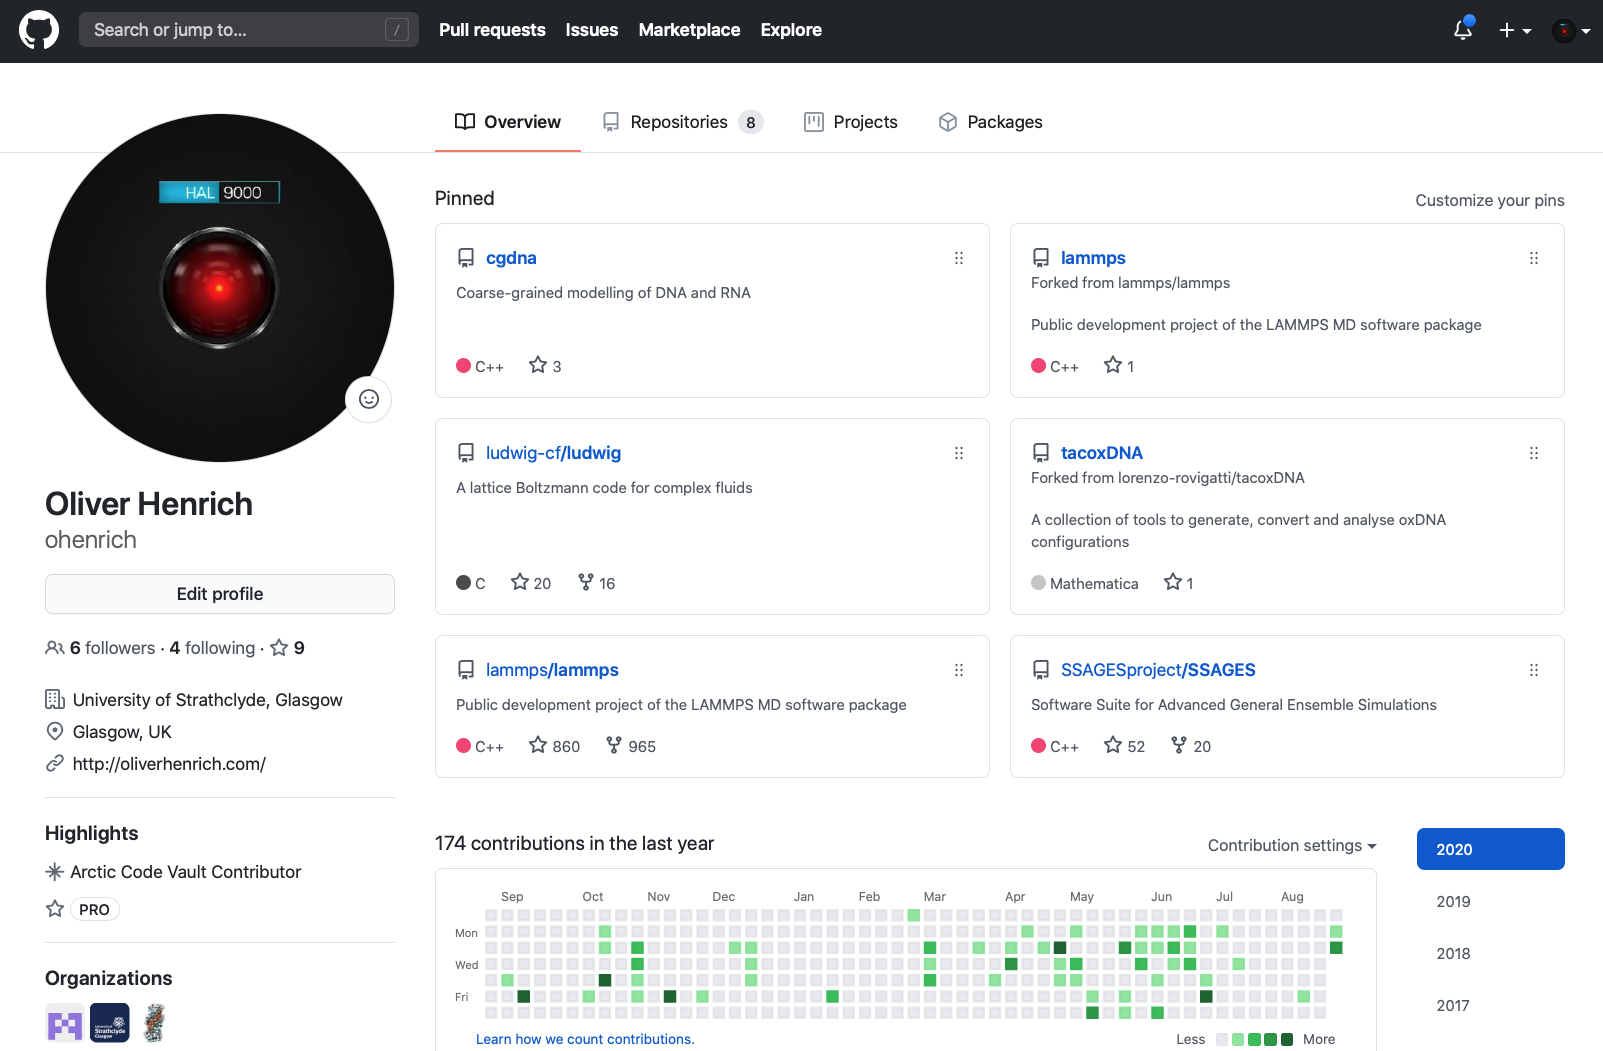
\includegraphics[width=0.75\textwidth]{sec3/github-myprofile.png}
  \end{figure}

\end{frame}

\begin{frame}[fragile]
\emptyframetitle

  On GitHub, create your first repository.\\[0.25cm]
  Go to \textbf{Repositories}
  \begin{figure}[h]
    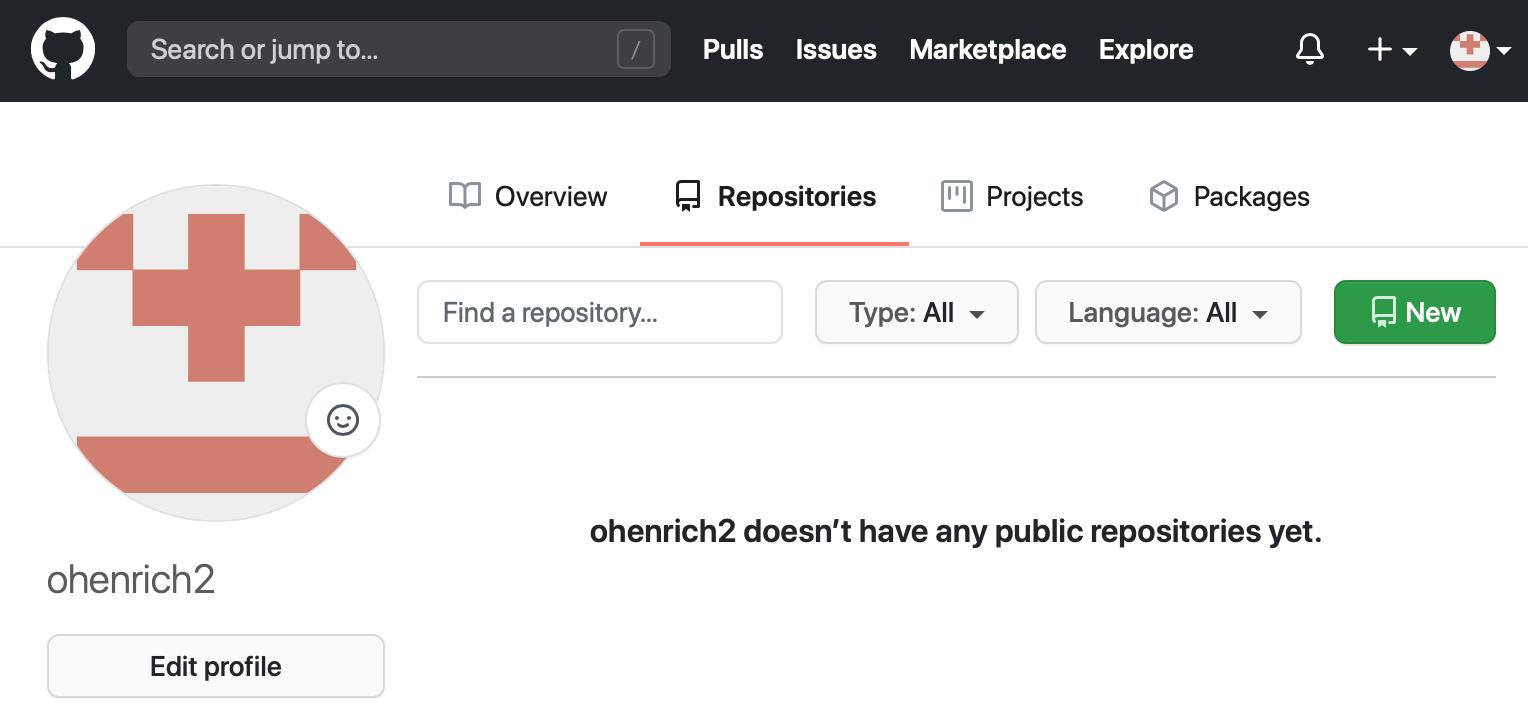
\includegraphics[width=0.75\textwidth]{sec3/github-new-repo.png}
  \end{figure}
  and click on the \textbf{New} button.

\end{frame}


\begin{frame}[fragile]
\emptyframetitle

  \begin{columns}

    \begin{column}{0.5\textwidth}
      Then chose a name for your repo and create it.
      \begin{figure}[h]
        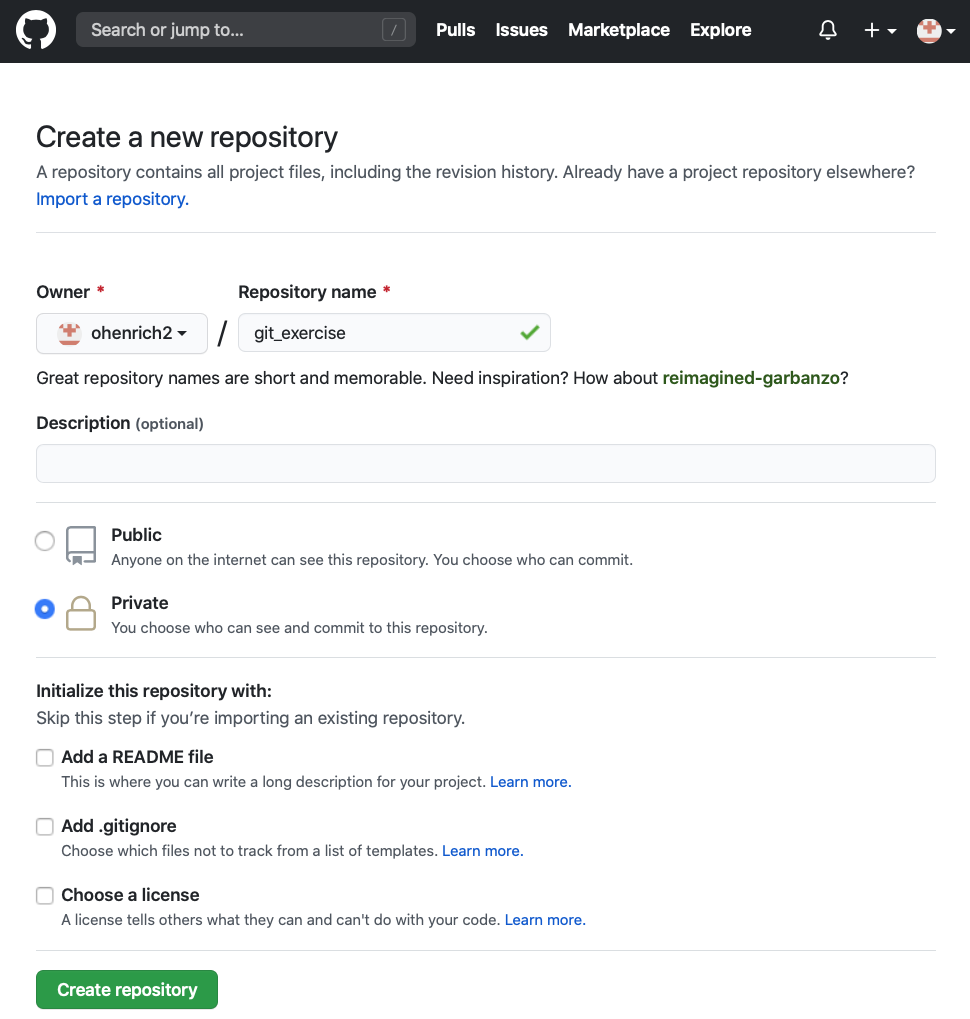
\includegraphics[width=0.95\textwidth]{sec3/github-create-new-repo.png}
      \end{figure}
    \end{column}

    \begin{column}{0.5\textwidth}
      There are a number of options:
      \begin{itemize}
        \item \textbf{Import a repository}: This option is only available if you have another \textit{remote} repo unlike the one you just created
        \item \textbf{Public / Private}: Choose private so only you can interact with it. You can give others access later on.
        \item \textbf{Initialize this repository with}: This adds certain files. Don't do this as we want to import your existing project.
      \end{itemize}
   
\vspace*{0.25cm}   Press the "Create repository" button.
    \end{column}
  \end{columns}

\end{frame}

\begin{frame}[fragile]
\emptyframetitle

  The next thing you get is a useful overview of what you might want to do next. It contains already the correct code with your individual username, repo URL, etc.

  \begin{columns}
  \begin{column}{0.6\textwidth}
    \begin{figure}[h]
      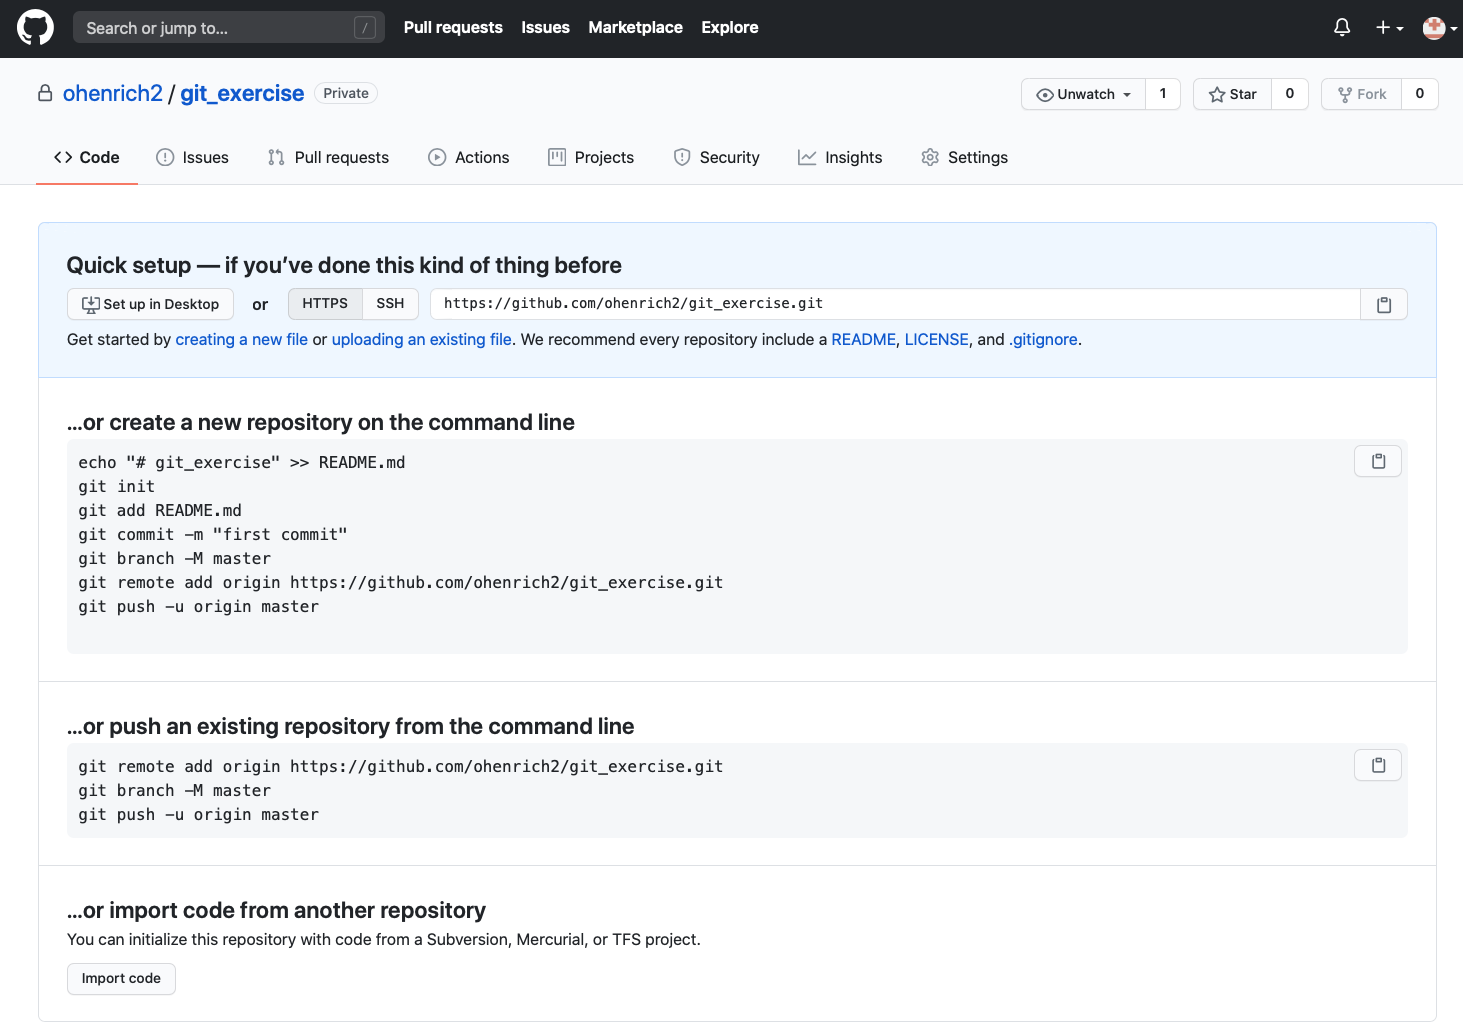
\includegraphics[width=1.0\textwidth]{sec3/github-quick-setup.png}
    \end{figure}
  \end{column}
  \begin{column}{0.4\textwidth}
    \vspace*{3.25cm}
    We are going to do option 2:\\ \textbf{"push an existing repository from the command line"}
  \end{column}
  \end{columns}

\end{frame}


\begin{frame}[fragile]
\emptyframetitle

  But let's first go back to your profile page and check your "Repositories".\\[0.25cm]

  \begin{figure}[h]
    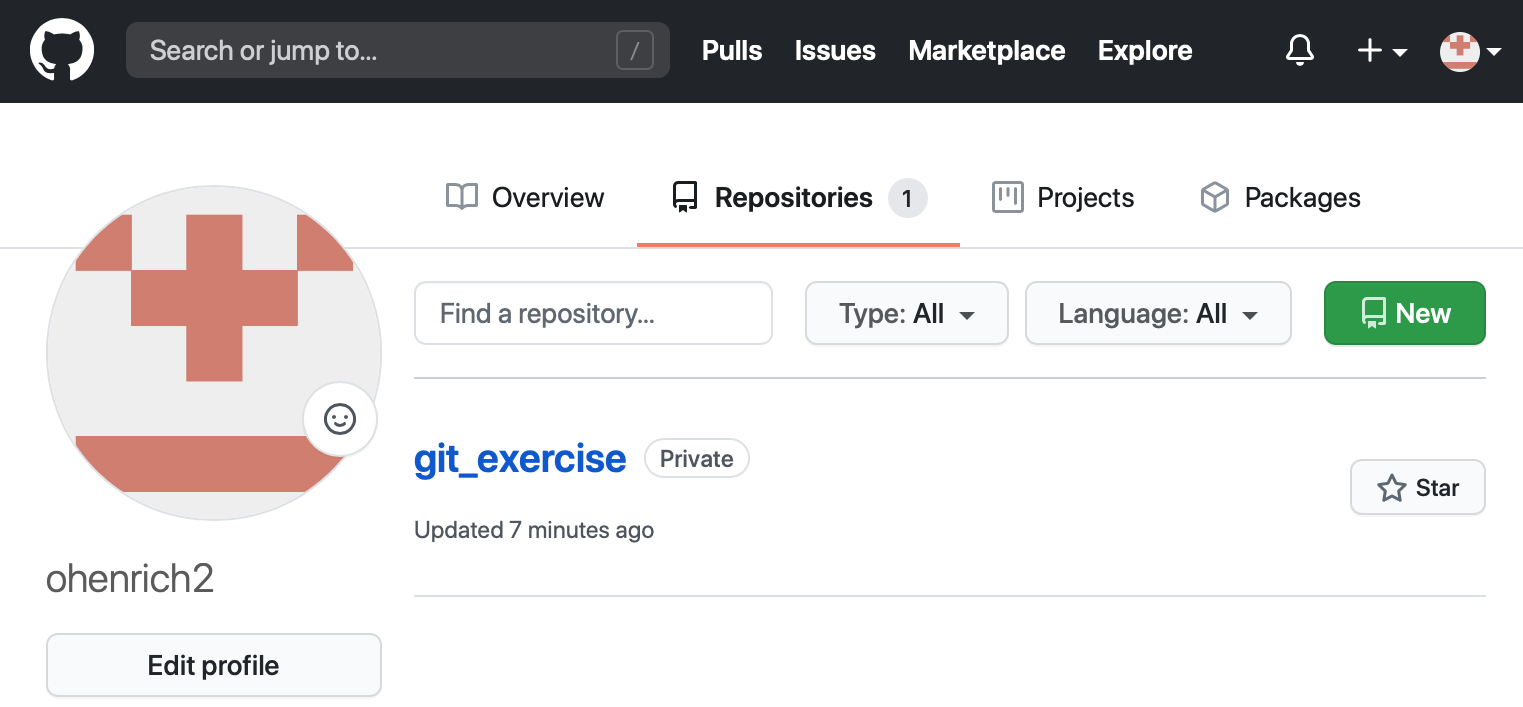
\includegraphics[width=0.75\textwidth]{sec3/github-new-repo-created.png}
  \end{figure}

  When you browse the content of your repo you will see it is completely empty.

\end{frame}


\begin{frame}[fragile]
\emptyframetitle

  Your current situation looks like this

  \begin{figure}[h]
    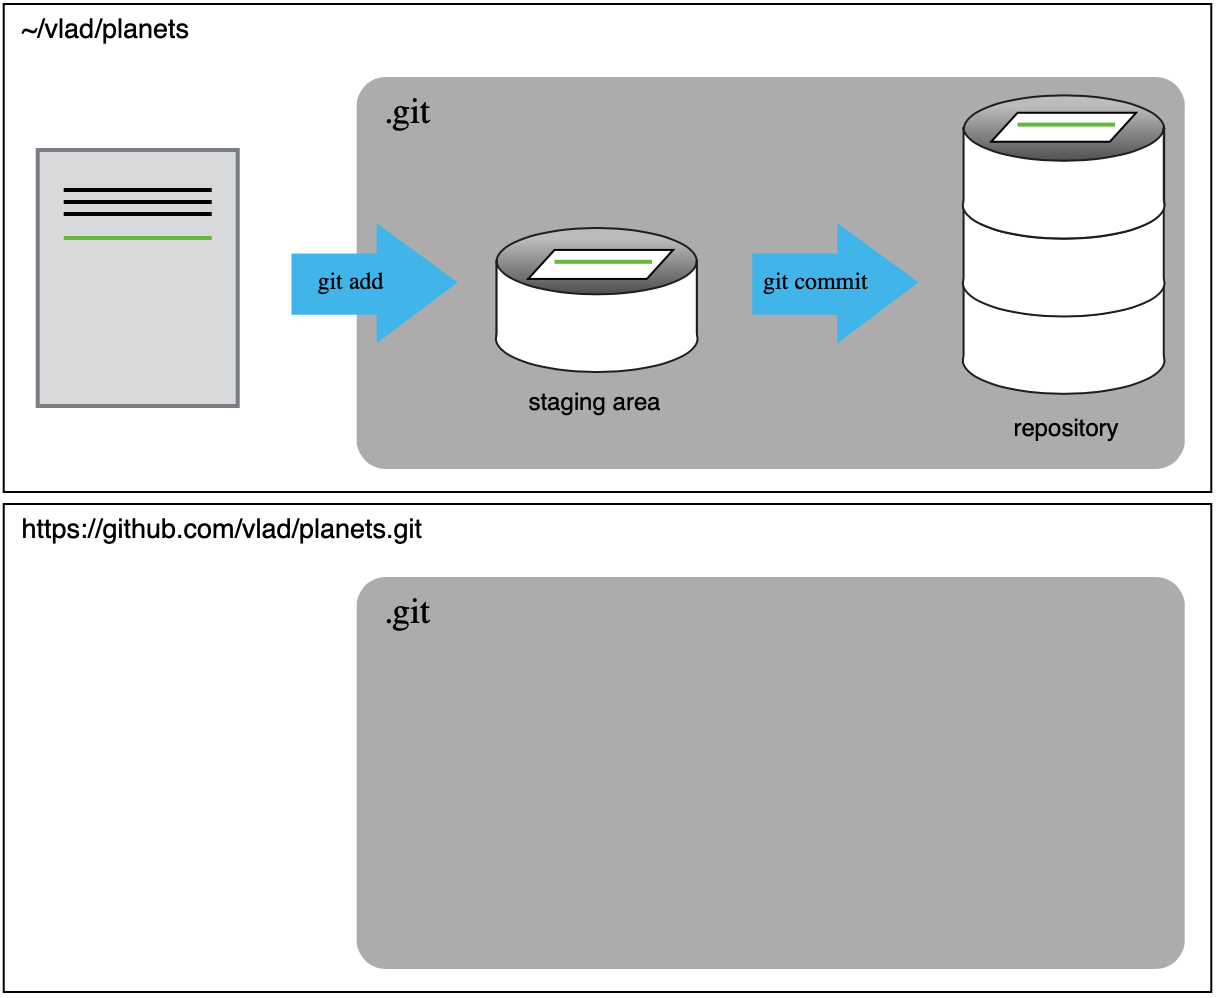
\includegraphics[width=0.55\textwidth]{sec3/git-prior-to-export.png}
  \end{figure}

  We will now \textbf{export your existing local} repo to the \textbf{newly created remote} repo on GitHub.

\end{frame}


\begin{frame}[fragile]
\emptyframetitle


  The full documentation is available on \textbf{\url{https://docs.github.com/en}}, under \textbf{GitHub.com $\rightarrow$ Importing your projects $\rightarrow$ Adding an existing project to GitHub using the command line}.\\[0.25cm]

  \textbf{On GitHub}, look up the URL of your remote repo.\\[0.25cm]

  \textbf{On the command line} change to the directory of your local repo and issue the following sequence of commands replacing username, etc accordingly.
  \begin{lstlisting}[language=bash]
    $ cd git_exercise
    $ git remote add origin https://github.com/username/repo_name.git
    $ git branch -M master
    $ git push -u origin master
  \end{lstlisting}

\end{frame}


\begin{frame}[fragile]
\emptyframetitle

  On GitHub check what's in your remote repository.
  \begin{figure}[h]
    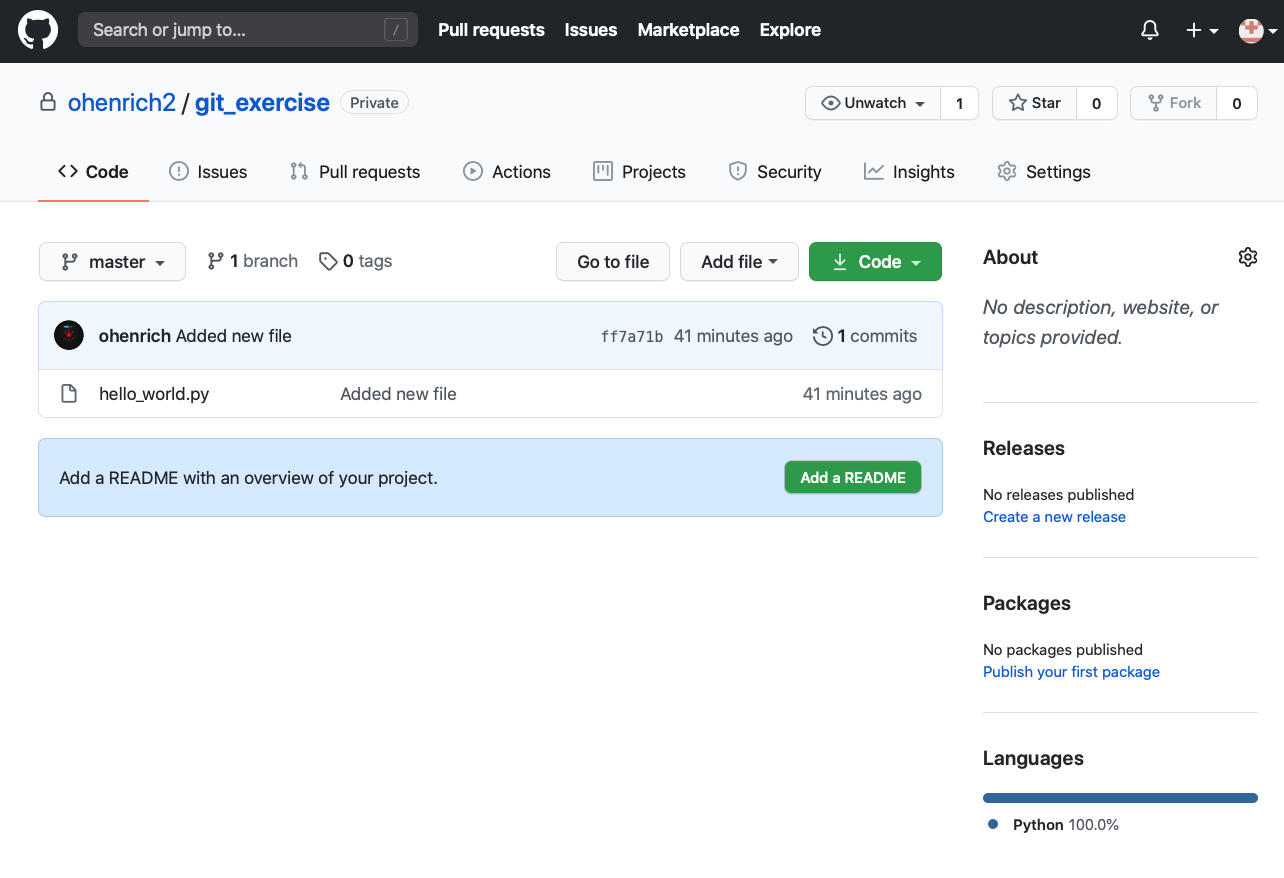
\includegraphics[width=0.85\textwidth]{sec3/github-pushed-existing-repo.png}
  \end{figure}
  \vspace*{-2.5cm}
  \textbf{Hooray!\\[0.25cm] Here is your local code making a\\ first appearance on GitHub!}

\end{frame}


\subsection{Collaborating On GitHub}\hypertarget{sec3.2}{}


\begin{frame}[fragile]
\emptyframetitle

  In \hyperlink{sec3.1}{Section 2.6} we \textbf{exported} an existing \textbf{\textit{local} repository} to your GitHub profile to \textbf{create a remote repository}.\\[0.35cm]

  The inverse process of \textbf{importing} an existing \textbf{\textit{remote} repository} from GitHub is called \textbf{cloning}.\\[0.35cm]

  \textbf{Cloning} produces a \textbf{local copy of the remote repository} on your machine. It requires 
  \begin{itemize}
    \item the \textbf{URL of the remote repository}
    \item the \textbf{\texttt{git clone}} command\\[0.35cm]
  \end{itemize}

  You can modify the local copy and \textbf{push the changes to the remote repository} on GitHub to share them with your collaborators. 
   
\end{frame}


\begin{frame}[fragile]
\emptyframetitle

  First navigate to the repository that you want to clone and click on the "Code" button

  \begin{figure}[h]
    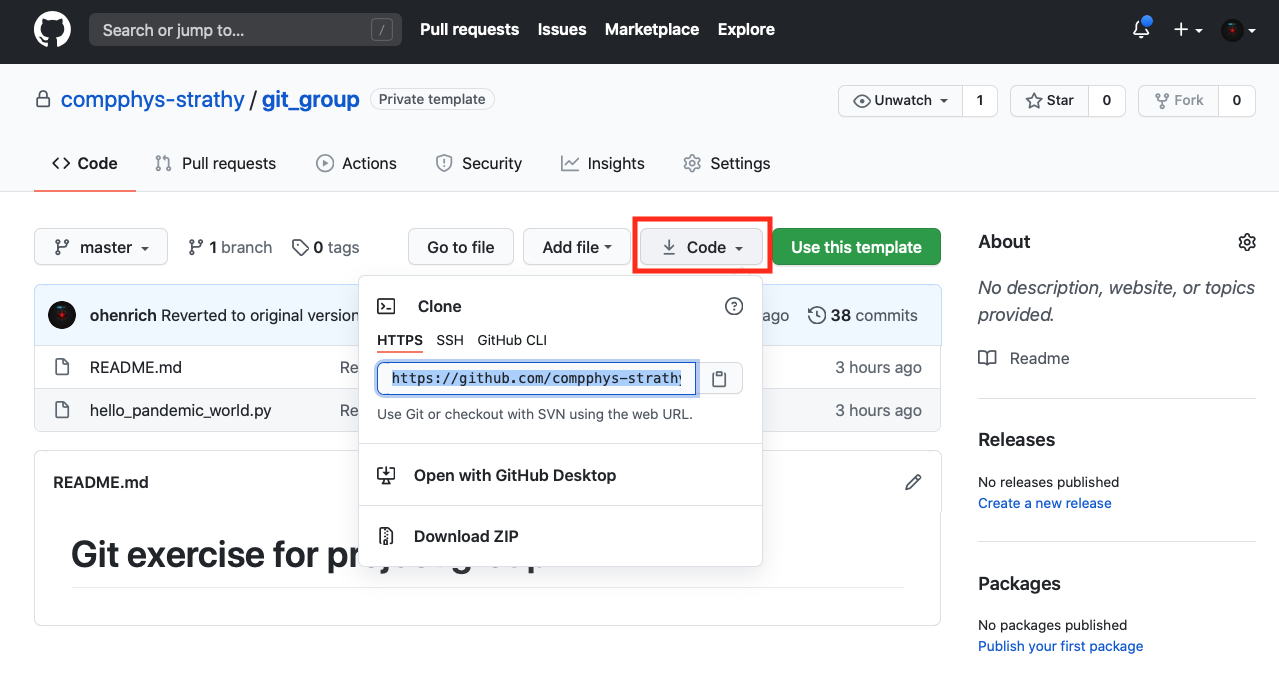
\includegraphics[width=0.75\textwidth]{sec3/github-clone.png}
  \end{figure}

  Copy the URL, e.g. by pressing the button next to it.

\end{frame}


\begin{frame}[fragile]
\emptyframetitle

  On your command line in your working directory issue the following command replacing \textbf{\texttt{URL}} with the actual URL:

  \begin{lstlisting}[language=bash]
    $ git clone URL 
  \end{lstlisting}

  \vspace*{-0.25cm}
  \begin{block}{Output of \texttt{git clone URL}}
  \vspace*{-0.25cm}
    \begin{lstlisting}[language=bash, basicstyle=\footnotesize\ttfamily]
      Cloning into 'git_group'...
      remote: Enumerating objects: 109, done.
      remote: Counting objects: 100% (109/109), done.
      remote: Compressing objects: 100% (79/79), done.
      remote: Total 109 (delta 33), reused 96 (delta 27), pack-reused 0
      Receiving objects: 100% (109/109), 14.32 KiB | 4.77 MiB/s, done.
      Resolving deltas: 100% (33/33), done.
    \end{lstlisting}
  \end{block}

  You can clone the repository it into a different name than the default name (the name on GitHub), e.g. \textbf{\texttt{blablabla}} by adding this after the URL. 

  \begin{lstlisting}[language=bash]
    $ git clone URL blablabla
  \end{lstlisting}
 
\end{frame}

\subsection{Conflicts}\hypertarget{sec3.3}{}

\begin{frame}[fragile]
\emptyframetitle

  \textbf{Conflicts} emerge when \textbf{several} people work on the \textbf{same} code and \textbf{update the remote repo}.\\[0.25cm]

  \begin{figure}[h]
    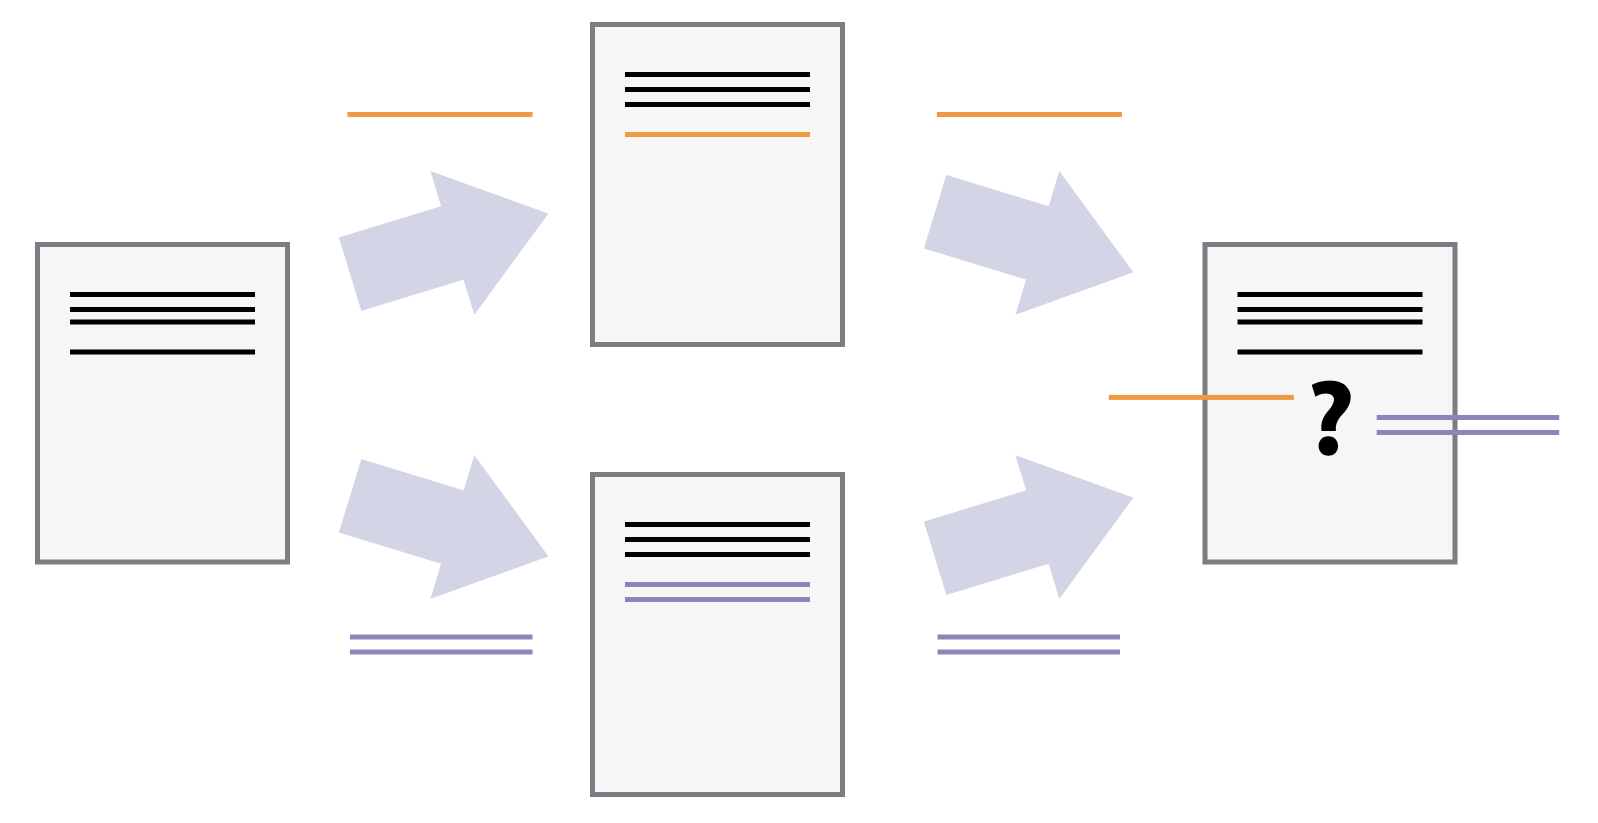
\includegraphics[width=0.7\textwidth]{sec3/git-conflict.png}
  \end{figure}

  The \textcolor{orange}{orange line} and the \textcolor{violet}{purple line} are approximately at the same position in the file. 

\end{frame}

\begin{frame}[fragile]
\emptyframetitle

  Let's look at our \texttt{Hello World!} example.\\[0.cm]

  \begin{columns}
    \begin{column}{0.5\textwidth}

      Your collaborator has checked in the following version:

      \begin{lstlisting}[language=python,basicstyle=\small\ttfamily]
        print('Hello World!')
        print('Hello Scotland!')
        print('Hello City of Glasgow!')
      \end{lstlisting}

    \end{column}

  \begin{column}{0.5\textwidth}

    Your version differs in the last line:
    \vspace{0.25cm}\\
    \begin{lstlisting}[language=python,basicstyle=\small\ttfamily]
      print('Hello World!')
      print('Hello Scotland!')
      print('Hello Greater Glasgow!')
    \end{lstlisting}

    \end{column}
  \end{columns}

  \begin{block}{Output of \texttt{git push origin master}}
    \begin{lstlisting}[language=bash, basicstyle=\tiny\ttfamily]
      To https://github.com/compphys-strathy/git_exercise.git
       ! [rejected]        master -> master (fetch first)
      error: failed to push some refs to 'https://github.com/compphys-strathy/git_exercise.git'
      hint: Updates were rejected because the remote contains work that you do
      hint: not have locally. This is usually caused by another repository pushing
      hint: to the same ref. You may want to first integrate the remote changes
      hint: (e.g., 'git pull ...') before pushing again.
      hint: See the 'Note about fast-forwards' in 'git push --help' for details.
    \end{lstlisting}
  \end{block}


\end{frame}

\begin{frame}[fragile]
\emptyframetitle

  What we have to do is \textbf{pull the changes from the remote repo} on GitHub into your local repo.\\[0.25cm]

  Git \textbf{tries to merge them automatically} into your local copy, and \textbf{if successful this can be pushed} to the remote repo on GitHub.

  \begin{lstlisting}[language=bash]
    $ git pull origin master
  \end{lstlisting}
  \vspace*{-0.25cm}
  \begin{block}{Output of \texttt{git pull origin master}}
    \begin{lstlisting}[language=bash, basicstyle=\tiny\ttfamily]
      remote: Enumerating objects: 5, done.
      remote: Counting objects: 100% (5/5), done.
      remote: Compressing objects: 100% (2/2), done.
      remote: Total 3 (delta 0), reused 0 (delta 0), pack-reused 0
      Unpacking objects: 100% (3/3), 682 bytes | 682.00 KiB/s, done.
      From https://github.com/compphys-strathy/git_exercise
       * branch            master     -> FETCH_HEAD
         dbd3016..5b9c121  master     -> origin/master
      Auto-merging hello_world.py
      CONFLICT (content): Merge conflict in hello_world.py
      <@\textbf{\textcolor{red}{Automatic merge failed; fix conflicts and then commit the result.}}@>
    \end{lstlisting}
  \end{block}

\end{frame}


\begin{frame}[fragile]
\emptyframetitle

  Check what Git has done to your local file.
 \vspace*{0.25cm} 
  \begin{columns}
    \begin{column}{0.59\textwidth}
      \begin{lstlisting}[language=python, basicstyle=\small\ttfamily]
        print('Hello World!')
        print('Hello Scotland!')
        <<<<<<< HEAD
        print('Hello Greater Glasgow!')
        =======
        print('Hello City of Glasgow!')
        >>>>>>> 5b9c121bac
      \end{lstlisting}
    \end{column}
    \begin{column}{0.41\textwidth}
      Our change is preceded by \texttt{\textbf{<<<<<<< HEAD}}.\\[0.2cm]
      Git inserted \texttt{\textbf{=======}} as separator between the conflicting changes.\\[0.2cm]
      The end of the content downloaded from GitHub is marked with \texttt{\textbf{>>>>>>>}}.
    \end{column}
  \end{columns}

  \vspace*{0.5cm}
  We need to \textbf{remove} these markers, \textbf{reconcile} the changes and \textbf{check in a new version}. 

\end{frame}


\begin{frame}[fragile]
\emptyframetitle

  \vspace*{-0.5cm}
  \begin{columns}
    \begin{column}{0.59\textwidth}
      \begin{lstlisting}[language=python, basicstyle=\small\ttfamily]
        print('Hello World!')
        print('Hello Scotland!')
        print('Hello Greater Glasgow!')
        print('Hello City of Glasgow!')
      \end{lstlisting}
    \end{column}
    \begin{column}{0.41\textwidth}
      \vspace*{0.5cm}\\
      We remove the markers and keep both lines.
    \end{column}
  \end{columns}

  Lets' first check the status.
  \vspace*{-0.25cm}

 \begin{columns}
    \begin{column}{0.59\textwidth}
      \begin{block}{Output of \texttt{git status} after editing}
        \begin{lstlisting}[language=bash, basicstyle=\tiny\ttfamily]
      git status
      On branch master
      Your branch and 'origin/master' have diverged,
      and have 2 and 1 different commits each, respectively.
        (use "git pull" to merge the remote branch into yours)

      You have unmerged paths.
        (fix conflicts and run "git commit")
        (use "git merge --abort" to abort the merge)

      Unmerged paths:
        (use "git add <file>..." to mark resolution)
              both modified:   hello_world.py
        \end{lstlisting}
      \end{block}
    \end{column}
    \begin{column}{0.41\textwidth}
      \vspace*{3.5cm}\\
      We are using the last option.
    \end{column}
  \end{columns}

\end{frame}

\begin{frame}[fragile]
\emptyframetitle

  \begin{lstlisting}[language=bash]
    $ git add hello_world.py 
    $ git commit -m 'Resolved conflict'
  \end{lstlisting}

  \vspace*{-0.25cm}
  \begin{block}{Output of \texttt{git commit}}
  \vspace*{-0.25cm}
    \begin{lstlisting}[language=bash]
      [master c7c8fb8] Resolved conflict
    \end{lstlisting}
  \end{block}
 
  \vspace*{-0.25cm}
  \begin{lstlisting}[language=bash]
    $ git push origin master 
  \end{lstlisting}

  \vspace*{0.25cm}

  \textbf{Minimise the number of conflicts by using this workflow}:

  \begin{enumerate}
    \item Update local \hspace*{0.25cm} \texttt{\textbf{git pull origin master}}
    \item Make changes	
    \item Stage changes \hspace*{0.25cm} \texttt{\textbf{git add your\_edited\_file.py}}
    \item Commit changes \hspace*{0.25cm} \texttt{\textbf{git commit -m "Your commit message"}}
    \item Update remote \hspace*{0.25cm} \texttt{\textbf{git push origin master}}
  \end{enumerate}

\end{frame}
